\newpage
\section{Graficzny projekt interfejsu użytkownika}

\subsection{Ekran logowania}
\noindent Pierwszym widokiem, który widzi użytkownik po wejściu na stronę jest ekran logowania. 
Na środku konterena znajduje się nazwa aplikacji, a pod nią formularz logowania. 
W celu potwierdzenia logowania należy kliknąć przycisk "Zaloguj się".
\begin{figure}[h]
    \centering
    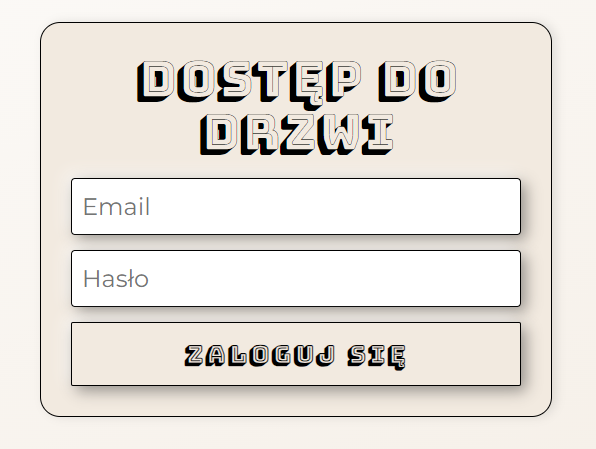
\includegraphics[scale=0.7]{photos/ekran_logowania.png}
    \caption{Ekran logowania}
    \label{fig:login}
\end{figure}

\noindent W przypadku niepoprawnego wprowadzenia danych, użytkownik zostanie poinformowany
 o błędnym formacie emaila:
\begin{figure}[h]
    \centering
    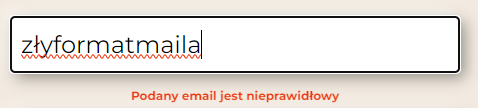
\includegraphics[scale=0.7]{photos/zlymail.png}
    \caption{Ekran logowania - błędny email}
    \label{fig:login}
\end{figure}

\noindent Analogicznie po wprowadzeniu błędnego hasła wyświetli się następujący komunikat:
\begin{figure}[h]
    \centering
    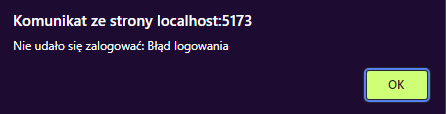
\includegraphics[scale=0.7]{photos/zle_haslo.png}
    \caption{Ekran logowania - błędne hasło}
    \label{fig:login}
\end{figure}
\newpage
\subsection{Profil pracownika}
Pracownik po zalogowaniu się do systemu zostanie przekierowany na strone swojego profilu,
gdzie zostają mu wyśwetlone informacje o nim:
\begin{figure}[h]
    \centering
    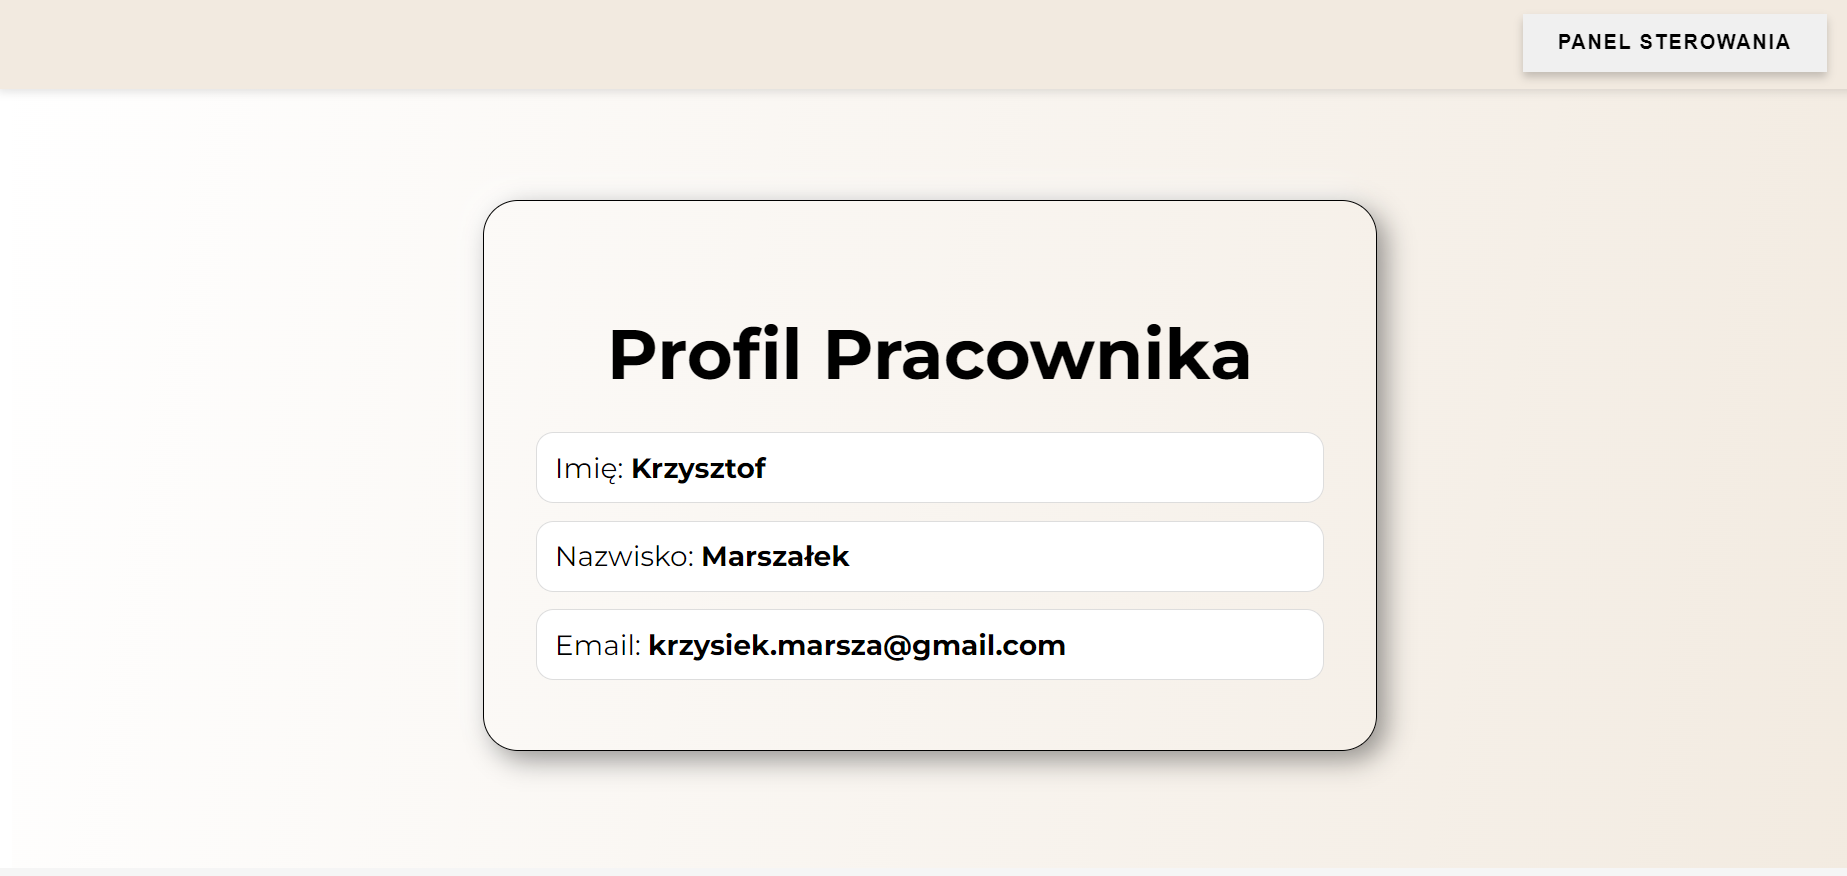
\includegraphics[scale=0.3]{photos/profil_pracownika.png}
    \caption{Profil pracownika}
    \label{fig:login}
\end{figure}


\noindent W prawym górnym rogu znajduje się tzw. hamburger menu pod nazwa "Panel sterowania", które po kliknięciu
rozwinie się i pokaże opcje, które są dostępne dla pracownika:
\begin{figure}[h]
    \centering
    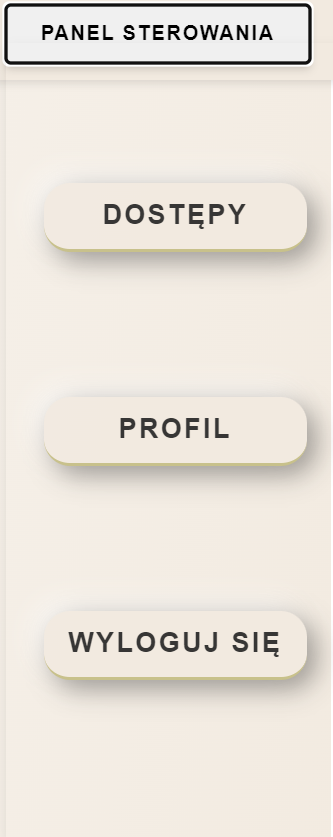
\includegraphics[scale=0.35]{photos/panel_sterowania_pracownika.png}
    \caption{Panel sterowania pracownika}
    \label{fig:login}
\end{figure}

\newpage

\noindent Po kliknięciu w opcje "Dostępy" zostanie wyświetlona lista dostępów do drzwi, które zostały przydzielone pracownikowi:
\begin{figure}[h]
    \centering
    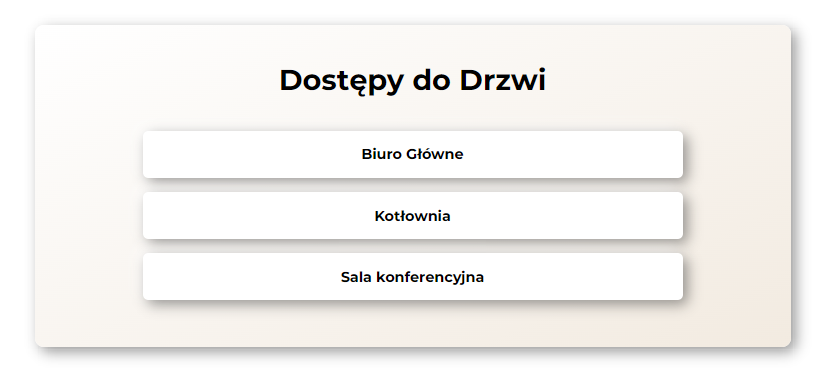
\includegraphics[scale=0.5]{photos/dostepy_do_drzwi_pracownika.png}
    \caption{Lista dostępów do drzwi pracownika}
    \label{fig:login}
\end{figure}

\subsection{Profil Administratora}
\noindent Administartor analogicznie jak pracownik po zalogowaniu zostanie przekierowany na stronę swojego profilu, 
natomiast panel sterowania będzie wyglądał następująco:
\begin{figure}[h]
    \centering
    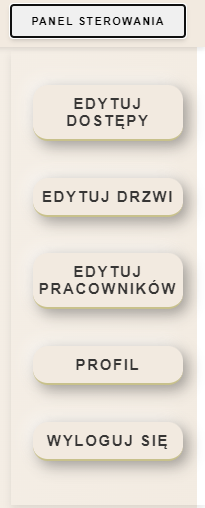
\includegraphics[scale=0.6]{photos/panel_sterowania_administratora.png}
    \caption{Panel sterowania administratora}
    \label{fig:login}
\end{figure}


\newpage

\subsubsection{Edyowanie dostępów}
\noindent Administrator po kliknięciu w opcje "Edytuj dostępy" zostanie przekierowany na stronę, gdzie będzie mógł edytować dostępy do drzwi.
Z listy wybieranej może wybrać pracownika, któremu chce zmienić dostęp do drzwi, a następnie z listy rozwijanej wybrać drzwi, które chce przydzielić pracownikowi.
Po kliknięciu w przycisk "Przydziel dostęp" zostanie zapisana zmiana w bazie danych. Poniżej 
znajduje się lista wszystkich dostępów do drzwi, które zostały przydzielone pracownikom. Administartor
może usunąć dostęp klikając w przycisk "Usuń".
\begin{figure}[h]
    \centering
    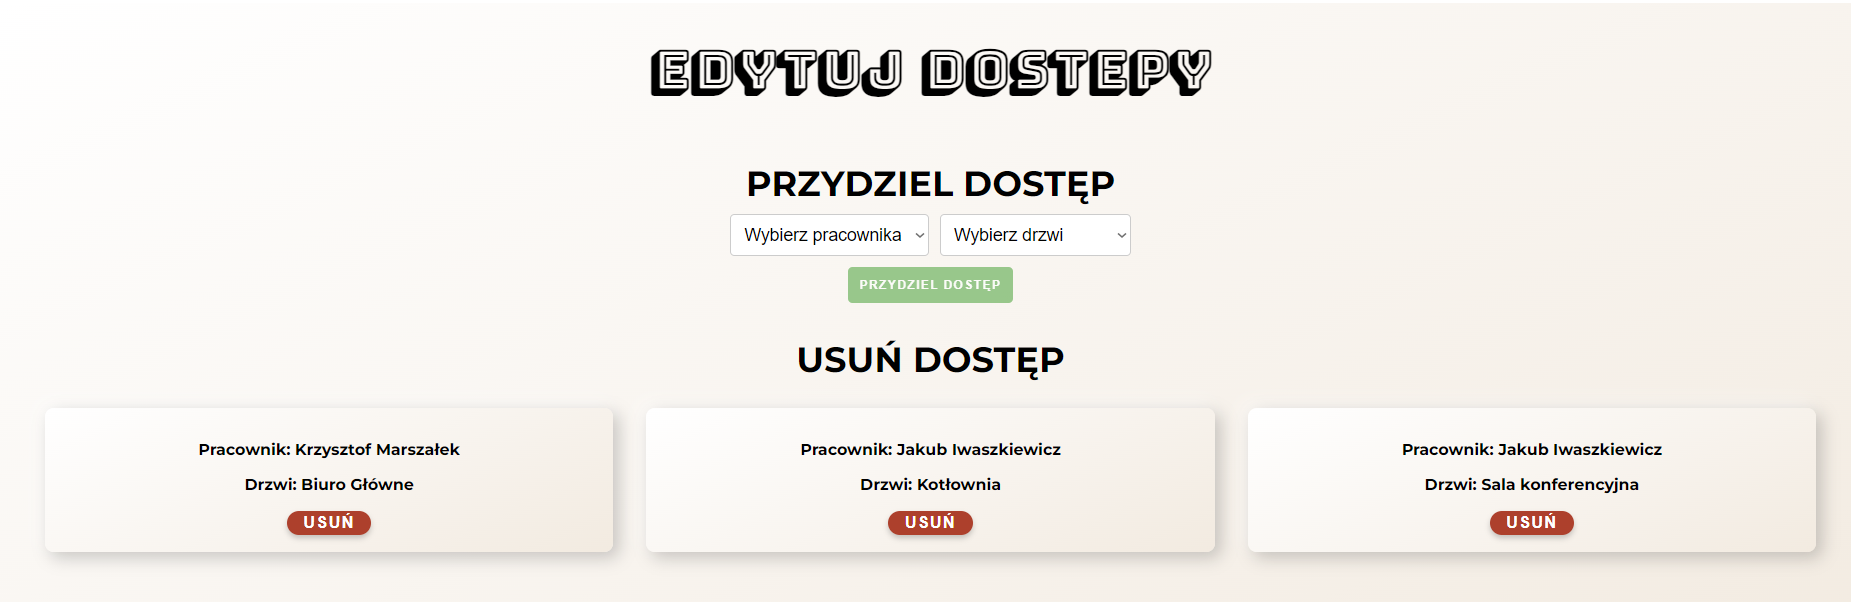
\includegraphics[scale=0.3]{photos/edytowanie_dostępów.png}
    \caption{Edytowanie dostępów}
    \label{fig:login}
\end{figure}


\subsubsection{Edytowanie drzwi}
\noindent Administrator po kliknięciu w opcje "Edytuj drzwi" zostanie przekierowany na stronę, 
gdzie będzie mógł edytować drzwi. Funkcjonalnośc dodawania drzwi wygląda w taki sposób, że administratorm
musi podać nazwę drzwi oraz jego opis. Po kliknięciu w przycisk "Dodaj" zostanie zapisana zmiana w bazie danych.
Poniżej znajduję się lista wszystkich drzwi z nazwami, które zostały dodane do systemu. Administrator może usunąć drzwi klikając w przycisk "Usuń".

\begin{figure}[h]
    \centering
    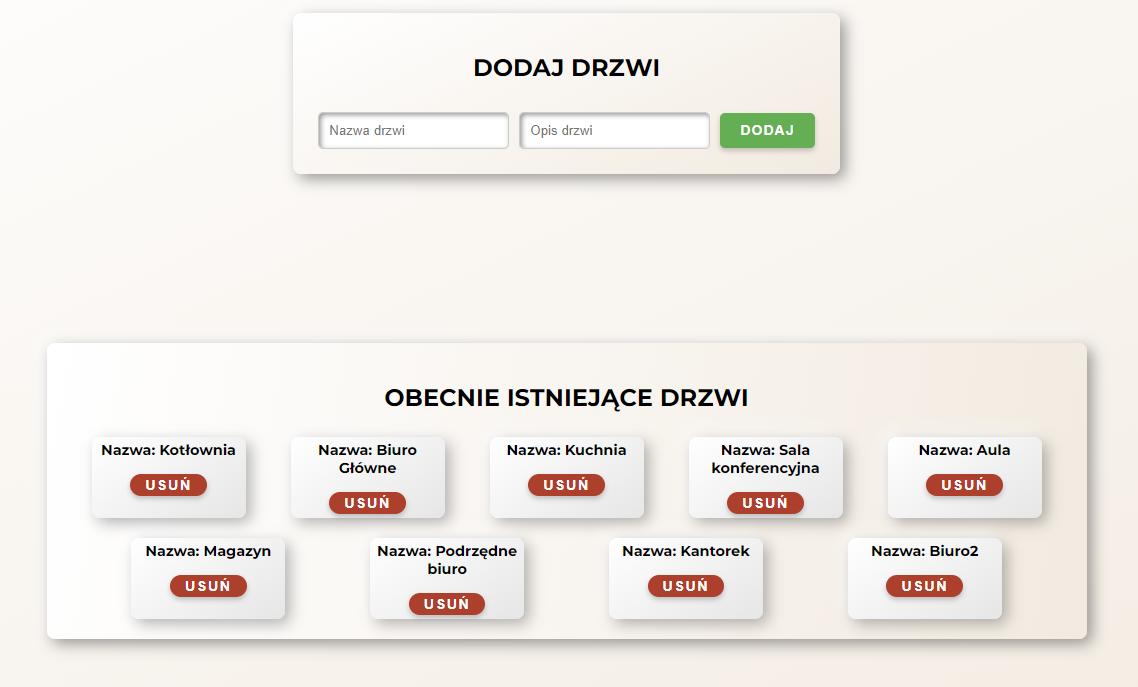
\includegraphics[scale=0.45]{photos/edytowanie_drzwi.png}
    \caption{Edytowanie drzwi}
    \label{fig:login}
\end{figure}

\subsubsection{Edytuj pracowników}
\noindent Administrator po kliknięciu w opcje "Edytuj pracowników" zostanie przekierowany na stronę,
gdzie będzie mógł edytować pracowników. Funkcjonalność dodawania pracownika
 wygląda w taki sposób, że administrator musi podać imię, nazwisko, email oraz hasło pracownika. 
 W każdej chwili może odsłonić hasło klikając przycisk "Pokaż hasło". Po kliknięciu 
 w przycisk "Dodaj pracownika" zostanie zapisana zmiana w bazie danych. Ponizej 
 znajduje się lista wszystkich pracowników, którzy zostali dodani do systemu.
  Administrator może usunąć pracownika klikając w przycisk "Usuń". W przypadku klinęcia usuń, wyskoczy 
  potwierdzenie usunięcia pracownika.
\begin{figure}[h]
    \centering
    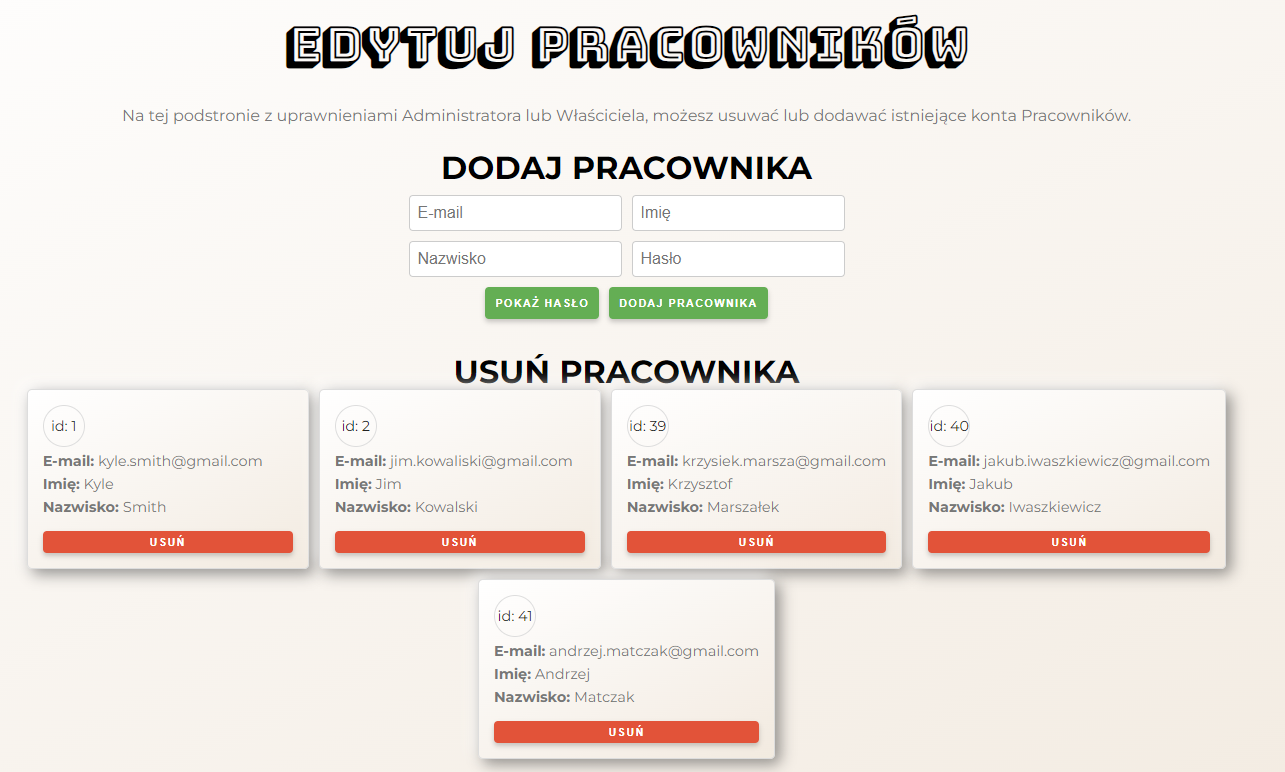
\includegraphics[scale=0.48]{photos/edytowanie_pracownikow.png}
    \caption{Edytowanie pracowników}
    \label{fig:login}

\end{figure}

\newpage

\subsection{Profil właściciela}
\noindent Właściciel analogicznie jak pracownik i administrator po zalogowaniu zostanie 
przekierowany na stronę swojego profilu. Właściciel ma dostęp do wszystkich opcji, które są dostępne 
dla administratora, oraz do dodatkowych opcji, takich jak "Dodaj przywileje" oraz "Usuń przywileje".

\begin{figure}[h]
    \centering
    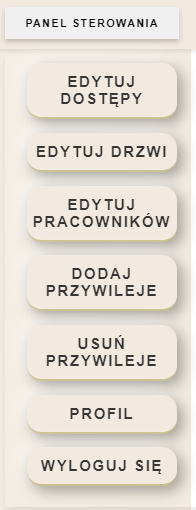
\includegraphics[scale=0.45]{photos/panel_sterowania_wlasciciela.png}
    \caption{Panel sterowania właściciela}
    \label{fig:login}
\end{figure}



\subsubsection{Edycja przywilejów}
\noindent Właściciel po kliknięciu w opcje "Edytuj przywileje" zostanie przekierowany na stronę,
na której może przyznać przywileje administratora wybranemu pracownikowi. Na tej podstronie zostaną 
wyświetleni wszyscy pracownicy. Właściciel może wybrać pracownika, któremu chce przyznać przywileje 
administratora. Po kliknięciu w przycisk "Dodaj jako Admina" zostanie zapisana zmiana w bazie danych.
W momecnie kiedy pracownik zostanie dodany jako administrator, mogą mu zostać przyznane przywileje właściciela.
\begin{figure}[h]
    \centering
    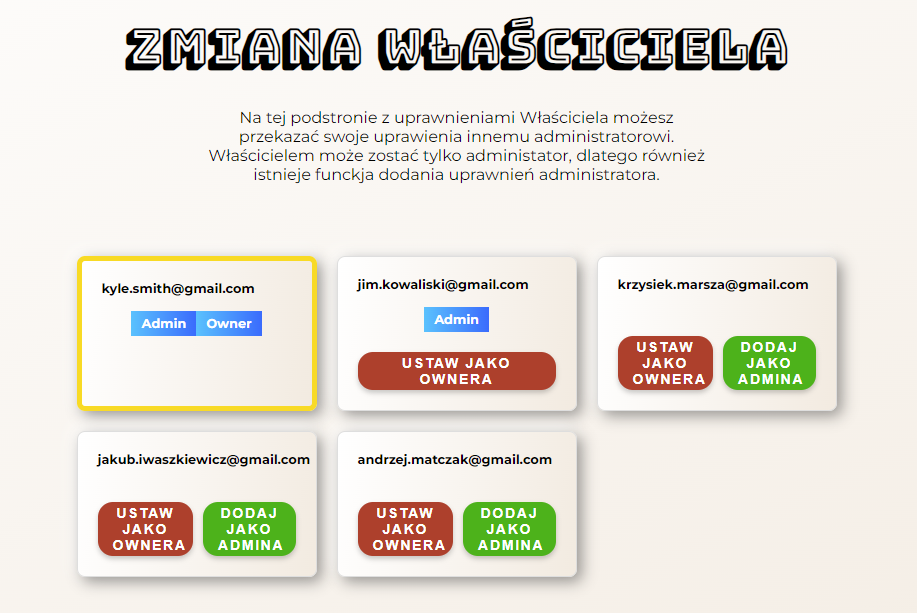
\includegraphics[scale=0.45]{photos/edytowanie_przywilejow.png}
    \caption{Edytowanie przywilejów}
    \label{fig:login}
\end{figure}
\newpage

\noindent W momencie kiedy właściciel przyzna przywileje administratora wybranemu pracownikowi, 
zostanie wyświetlony popout, który pyta właściciela czy chce przyznać przywileje właściciela wybranemu pracownikowi. Po 
kliknięciu w przycisk "Tak" zostanie zapisana zmiana w bazie danych.

\begin{figure}[h]
    \centering
    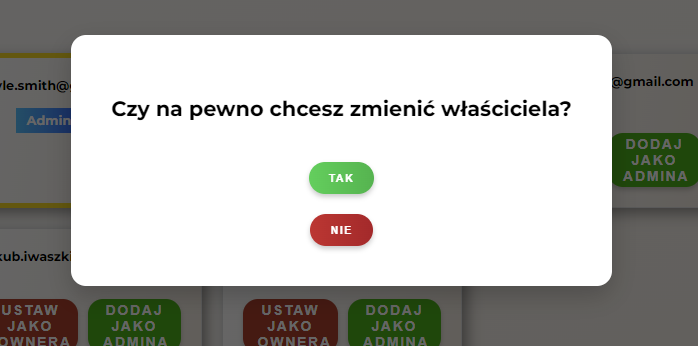
\includegraphics[scale=0.45]{photos/potwierdzenie.png}
    \caption{Potwierdzenie zmiany właściciela}
    \label{fig:login}
\end{figure}

\subsubsection{Usuwanie przywilejów}
\noindent Właściciel po kliknięciu w opcje "Usuń przywileje" zostanie przekierowany na stronę,
na której może usunąć przywileje administratora wybranemu pracownikowi. Na tej podstronie zostaną
wyświetleni wszyscy pracownicy z uprawieniami administratora. Właściciel może wybrać pracownika, któremu chce usunąć przywileje klikając
przycisk "Odbierz uprawnienia". Po kliknięciu w przycisk "Usuń jako Admina" zostanie zapisana zmiana w bazie danych:
\begin{figure}[h]
    \centering
    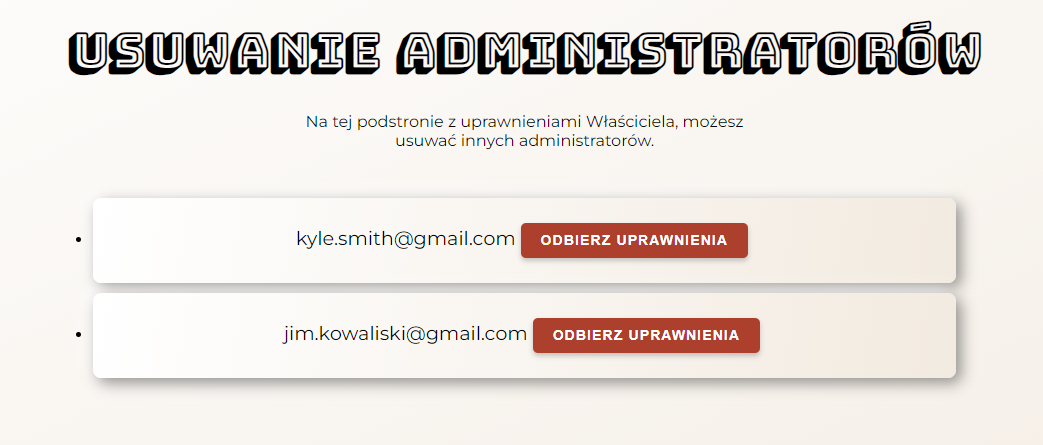
\includegraphics[scale=0.45]{photos/usuwanie_przywilejow.png}
    \caption{Usuwanie przywilejów}
    \label{fig:login}
\end{figure}